\setlength\abovedisplayskip{0.4pt}
\setlength\belowdisplayskip{0.4pt}

\chapter{Trigger development and performance}

\section{Introduction to triggering}

Modern "triggering" methods began with Walther Bothe's development of the coincidence method. In 1923 Bothe and Hans Geiger performed experiments on recoil electrons from Compton scattering. It was observed that there was a strong correlation between the trajectory of the recoil electron and that of the scattered photon. The correlation exhibited conservation of energy, conservation of momentum, and was consistent with the quantisation of energy. 

Bruno Rossi improved on Bothe and Geiger's photography based equipment with an electrical circuit. The coincidence ciruit accepts two inputs. If these inputs are recieced within the same time window, approximating coincidence, the circuit passes an output. Figure \ref{fig:ross} is the diagram of a coincidence circuit \cite{Bonolis:2011ph}. 
\begin{figure}[h!]
\begin{centering}
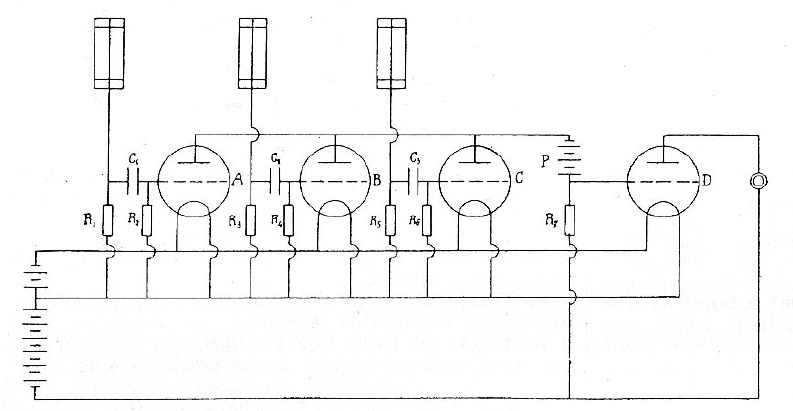
\includegraphics[width=4in]{Chapter5/importfigs/Rossis-coincidence-circuit-appearing-in-Ref-65-The-selecting-resistance-on-the-right.png}
\par\end{centering}
\caption{Rossi circuit with three Geiger-Muller coincidence circuits \cite{Bonolis:2011ph} \label{fig:ross}}
\end{figure}
Notice that there are three transistors that are each connected to a muon detector. These three transistors are in series with each other, but are in parallel with a fourth transistor. A signal registers when current passes through this fourth transistor. To open the fourth transistor, all three of the muon detectors must fire within a given time interval specified by the transistors.

The first coincidence circuits were used in cosmic ray experiments as higher frequency alternative to ion cloud chambers. 

\section{Triggering at CMS}

At stable beams, the LHC delivers bunch crossings every 25 nanoseconds. Each bunch crossing in turn will have some 20 hadron collisions. The resulting interaction rate -- $10^9$ interactions per second -- is orders of magnitude greater than the frequency that events can be written to disk, $10^2$ events per second. CMS therefore needs a means of filtering out the most interesting $10^2$ interactions per second while declining the other $10^6$ interactions per second. 

CMS uses a two-tiered triggering system. The first tier, the L1 trigger, is hardware based. The second tier, the high-level trigger (HLT), is software based. The L1 trigger recieves raw data from the calorimeters and the muon detectors; this determines when the tracker will readout data. The raw data from the tracker, calorimeters, and muon detectors is then passed on to a computer farm running the HLT menu. The HLT then performs a simplistic reconstruction of the raw data into physics objects useful for analysis: jets, tracks, and identifiable particles. If an event passes the HLT, the raw data is permanently stored in preparation for a more complex reconstruction \cite{Dasu:2000ge}\cite{Sphicas:2002gg}. 

\begin{figure}[h!]
\begin{centering}
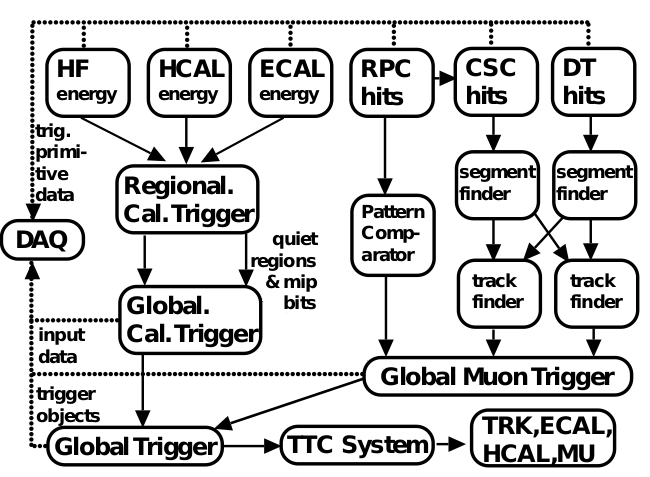
\includegraphics[width=4in]{Chapter5/importfigs/l1_trigger_flow.png}
\par\end{centering}
\caption{Flow of information in L1 trigger \label{fig:l1TriggerFlow}}
\end{figure}

The initial interaction rate is approximately $3.2$ $\mu s$. The L1 trigger can only pass some 1 in 1000 interactions to the HLT. The L1 trigger menu has an output rate of approximately 100 kHz. L1 achieves this rate by only considering data of reduced granularity and reduced resolution. A buffer is used to store the full event data while the L1 runs. The HLT menu reduces this to about 100 Hz as required by the limit on disk writing.

\begin{figure}[h!]
\begin{centering}
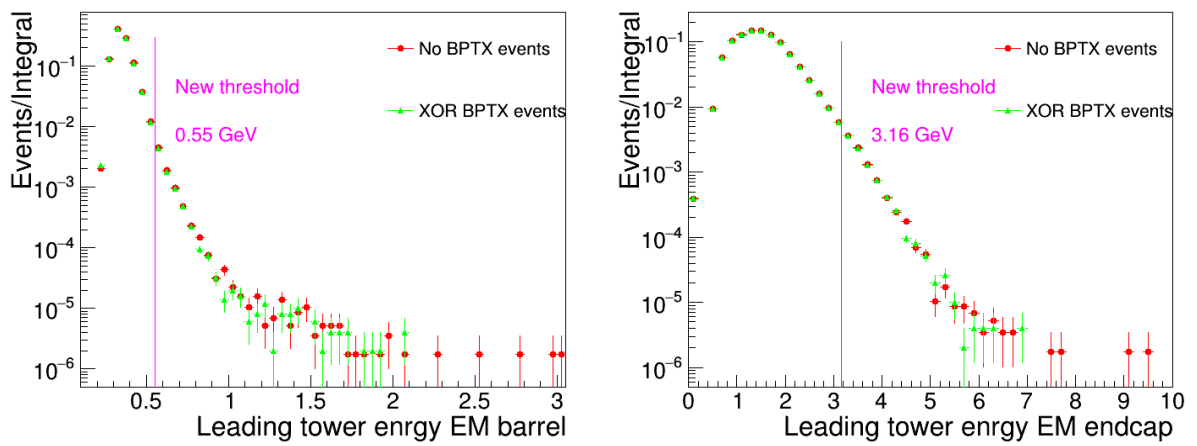
\includegraphics[width=6in]{Chapter5/importfigs/hf_max_tower.png}
\par\end{centering}
\caption{Leading tower energy distribution in HF \label{fig:hfMaxTower}}
\end{figure}

The 2015 UPC triggers were for low multiplicity events and low transverse momentum events. Typical heavy-ion collisions are high multiplicity events. Hard scattering dominates. Fig.\ref{fig:eventdisplayHI} is an event display of one of the first heavy-ion collisions at CMS in 2010.

\begin{figure}[h!]
\begin{centering}
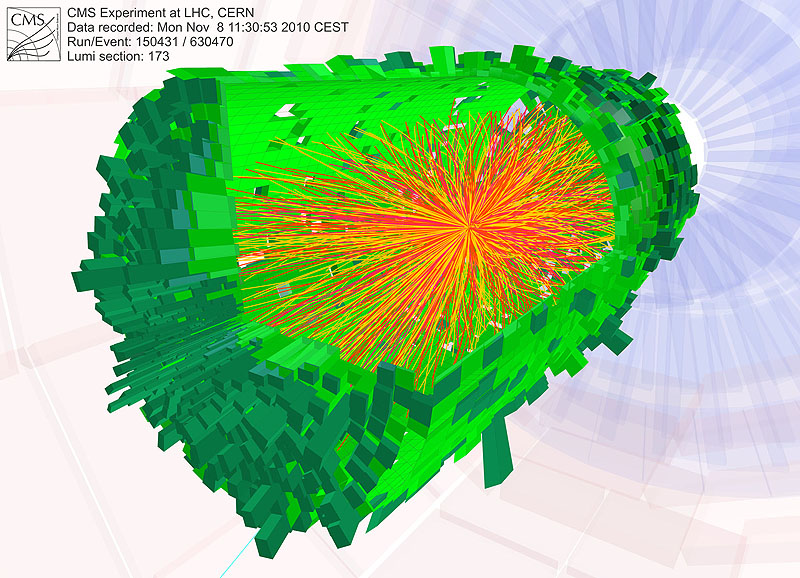
\includegraphics[width=4in]{Chapter3/importfigs/cms_firstleadcoll.jpg}
\par\end{centering}
\caption{High multiplicity PbPb collision \label{fig:eventdisplayHI}}
\end{figure}

Fig.\ref{fig:eventdisplayUPCUps} is the event display of a UPC upsilon candidate. Notice that there are only two reconstructed tracks, and that CMS is otherwise empty in all calorimeters. These events consitute a complement to those passing conventional more heavy-ion triggers. However, for Run-2 the Pb-Pb luminosities are high enough that UPC final states can be studied over a wide range of rapidity and $p_T$.

\begin{figure}[h!]
\begin{centering}
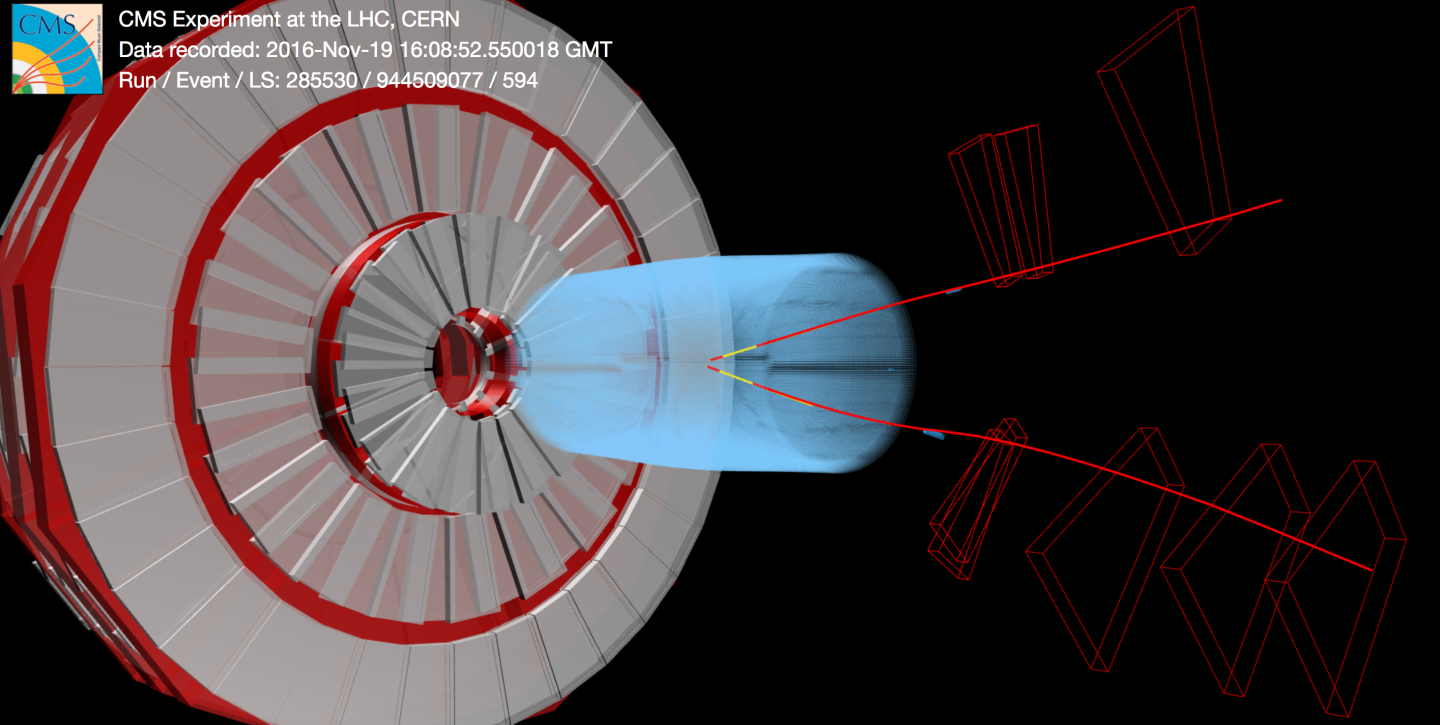
\includegraphics[width=4in]{Chapter3/importfigs/upcJpsi_run285530_lumi594_event944509077_v0.png}
\par\end{centering}
\caption{UPC Upsilon candidate \label{fig:eventdisplayUPCUps}}
\end{figure}

For this analysis, the L1 trigger applies two selections. First, the L1 checks that at least one of the HF is empty. This is the most important part of the trigger in so far as it suppressed the hadronic contamination of the dataset. Then, if there is at least 5 GeV of energy deposited in the ECAL, the event passes to the HLT. 

Low multiplicity events are difficult to distinguish from background. To compensate, the HLT in turn requires that there be at least once reconstructed track from the pixel tracker, to make sure that there are particles that will be reconstructed by the complete tracker. Only the pixel tracker is used for these HLTs to increase the speed of reconstruction while decreasing needed computer cycles. 

\section{Author's contributions}

\subsection{Pb+Pb 2015 UPC Triggers}
In preparation for the 2015 heavy-ion run and the 2016 p-Pb run, I prepared high-level trigger menus for the CMS Forward-HI group. This trigger menu was optimized for firing on ultra-peripheral collisions. I tested the menu's performance on Monte Carlo generated by STARLIGHT and reconstructed through a GEANT4 simulation of CMS. During the experiment, I was present at CERN to monitor the trigger rates and deliver daily reports on their performance. 

CMSSW includes an emulator for the L1 trigger. This software can re-emulate alternative L1 menus on previously taken CMS data. The performance of a trigger on the 2011 PbPb data, taken at $\sqrt{s_NN} = 2.7 TeV$ is extrapolated to the higher energy, $\sqrt{s_NN} = 5.2 TeV$, of the 2015 PbPb run.

I tested my HLT menu on both STARLIGHT MC and on data from the 2011 Pb+Pb run. STARLIGHT is a MC generator for ultra-peripheral collisions, in particular for the vector-meson photoproduction channels. I used STARLIGHT to generate MC sets for $Pb+Pb\rightarrow J/\Psi+Pb+Pb$ and $Pb+Pb\rightarrow \Upsilon(1s)+Pb+Pb$. I then used CMSSW to test the performance of the component bits of the HLT paths with respect to these MC sets. 

\begin{figure}[h!]
\begin{centering}
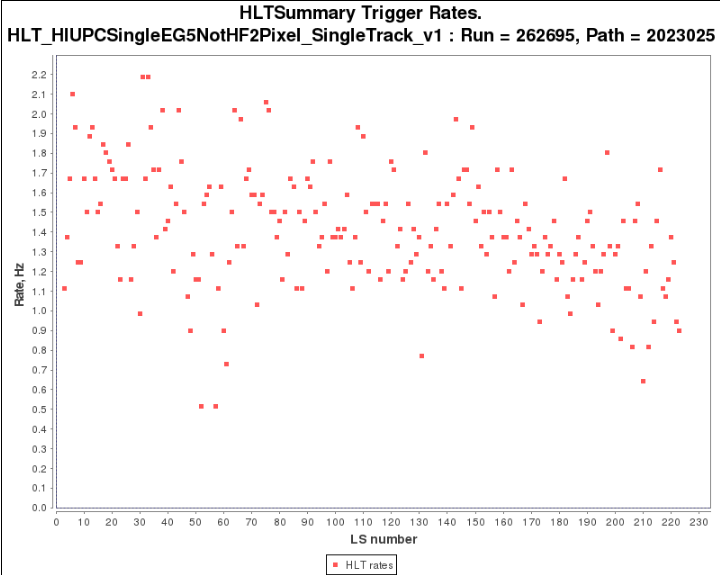
\includegraphics[width=4in]{Chapter5/importfigs/triggerRateExample.png}
\par\end{centering}
\caption{Example of trigger rate. \label{fig:trigRate}}
\end{figure}

It was my duty to carefully observe the state of the UPC triggers during the heavy-ion run. If the total HLT rate ever drifted above 100 Hz, the HLT menu could crash and CMS lose considerable data. It was important for the trigger contacts to make sure that there HLT paths were behaving stablely. I also analyzed express physics data to test that the vector-meson triggers saw appropriate mass resonances.

% Please add the following required packages to your document preamble:
% \usepackage{booktabs}
\begin{table}[h!]
\centering
\caption{L1 Trigger Average Rates for Run 263757}
\label{my-label}
\begin{tabular}{@{}l|p{1.6cm}|p{1.6cm}|p{1.6cm}|p{1.6cm}|p{1.3cm}|p{1.3cm}|}
%\begin{tabular}{@{}lllllll@{}}
\toprule
L1 Type                           & Pre-DT Rate (Hz) & Pre-DT RMS Rate (Hz) & Post-DT Rate (Hz) & Post-DT RMS Rate (Hz) & Initial Prescale & Final Prescale \\ \midrule
Double muon + HF veto (thresh. 1) & 7.78             & 8.39                 & 7.64              & 8.24                  & 0                & 0              \\
Double muon + HF veto (thresh. 2) & 7.86             & 8.49                 & 7.71              & 8.33                  & 0                & 0              \\
Single muon + HF veto (thresh. 2) & 85.58            & 89.76                & 84.31             & 88.53                 & 0                & 0              \\
Double EG2 + HF veto (thresh. 2)  & 2.26             & 2.62                 & 2.19              & 2.54                  & 0                & 0              \\
Single EG5 + HF veto (thresh. 2)  & 13.71            & 16.13                & 10.8              & 13.14                 & 0                & 0              \\ \bottomrule
\end{tabular}
\end{table}

% Please add the following required packages to your document preamble:
% \usepackage{booktabs}
\begin{table}[h!]
\centering
\caption{HLT Average Rates for Run 263757}
\label{my-label}
\begin{tabular}{@{}lll@{}}
\toprule
HLT Type             & L1 Seed                           & Average Rate of HLT (Hz) \\ \midrule
L1 pass through      & Double muon + HF veto (thresh. 1) & 7.64                     \\
Requires pixel track & Double muon + HF veto (thresh. 1) & 1.09                     \\
L1 pass through      & Double muon + HF veto (thresh. 2) & 7.71                     \\
Requires pixel track & Double muon + HF veto (thresh. 2) & 1.11                     \\
L1 pass through      & Single muon + HF veto (thresh. 2) & 22.41                    \\
Requires pixel track & Single muon + HF veto (thresh. 2) & 11.18                    \\
L1 pass through      & Double EG2 + HF veto (thresh. 2)  & 2.19                     \\
Requires pixel track & Single EG5 + HF veto (thresh. 2)  & 3.96                     \\ \bottomrule
\end{tabular}
\end{table}

\subsection{p+Pb 2016 UPC Triggers}

For the 2016 $p+Pb$ run I prepared a trigger menu similar to that of the 2015 $Pb+Pb$ run.

\begin{table}[h!]
\centering
\caption{L1 Trigger Average Rates for Run 285530}
\label{my-label}
\begin{tabular}{@{}l|p{1.6cm}|p{1.6cm}|p{1.6cm}|}
%\begin{tabular}{@{}lllllll@{}}
\toprule
L1 Type                           & Pre-DT Rate Before Prescale (Hz) & Pre-DT Rate After Prescale (Hz) & Post-DT Rate (Hz) \\ \midrule
Double muon + HF veto (1 Tower) & 5.47             & 5.47                 & 5.38            \\
Double muon + HF veto (2 Tower) & 5.47             & 5.47                 & 5.38            \\
Single muon + HF veto (1 Tower) & 123.31	       & 123.31               & 121.15          \\
Single muon + HF veto (2 Tower) & 123.31           & 123.31               & 121.15             \\
Double EG2 + HF veto (1 Tower)  & 228.22           & N/A                  & N/A            \\
Double EG2 + HF veto (2 Tower)  & 228.22           & N/A                  & N/A            \\
Single EG5 + HF veto (1 Tower)  & 211.17           & 211.17                & 207.00	              \\ 
Single EG5 + HF veto (2 Tower)  & 211.17           & 211.17                & 207.00	              \\ 
\bottomrule
\end{tabular}
\end{table}

\begin{table}[h!]
\centering
\caption{HLT Average Rates for Run 285530}
\label{my-label}
\begin{tabular}{@{}lll@{}}
\toprule
HLT Type             & L1 Seed                           & Average Rate of HLT (Hz) \\ \midrule
L1 pass through      & Double muon + HF veto (1 Tower) & 5.40	                    \\
Requires pixel track & Double muon + HF veto (1 Tower) & 1.20	                    \\
L1 pass through      & Double muon + HF veto (2 Tower) & 5.40                     	\\
Requires pixel track & Double muon + HF veto (2 Tower) & 1.20                     	\\
L1 pass through      & Single muon + HF veto (1 Tower) & 121.70                   	\\
Requires pixel track & Single muon + HF veto (1 Tower) & 58.16                    	\\
L1 pass through      & Single muon + HF veto (2 Tower) & 121.70	                    \\
Requires pixel track & Single muon + HF veto (2 Tower) & 58.16                    	\\
L1 pass through      & Double EG2 + HF veto (1 Tower)  & N/A                     	\\
Requires pixel track & Double EG2 + HF veto (1 Tower)  & N/A                     	\\
L1 pass through      & Double EG2 + HF veto (2 Tower)  & N/A                  		\\
Requires pixel track & Double EG2 + HF veto (2 Tower)  & N/A                     	\\ 
L1 pass through      & Single EG5 + HF veto (1 Tower)  & 208.18          			\\
Requires pixel track & Single EG5 + HF veto (1 Tower)  & 159.79                     \\
L1 pass through      & Single EG5 + HF veto (2 Tower)  & 208.18                     \\
Requires pixel track & Single EG5 + HF veto (2 Tower)  & 159.79	                    \\ \bottomrule
\end{tabular}
\end{table}

\section{Studies from trigger menus}

The UPC HLTs I designed are fruitful for a variety of physics studies. In addition to the coherent dijet study that is the subject of this thesis, the data gathered through the 2015 trigger menu can address UPC photoproduction of coherent and incoherent $J/\Psi$, coherent $\Psi(2s)$, coherent $\rho^0$, and possible $\rho^0$ excited states. The 2016 trigger menu is uniquely suited for studying exclusive vector meson photoproduction off the proton in p-Pb UPC. All of these studies have the potential for expanding our knowledge of the nuclear gluon PDFs at small-x, from $~10^-2$ to $~10^-5$.  
